\documentclass[10pt,letterpaper]{article}

\usepackage[margin=.5in]{geometry}
%\usepackage{xfrac}
\usepackage{polynom}
\usepackage{tikz}
\usepackage{amsmath}

\usetikzlibrary{calc}
\newcommand{\tikzmark}[1]{\tikz[overlay,remember picture] \node (#1) {};}
\DeclareMathOperator{\cis}{cis}
\newcommand{\jhat}{\hat{\jmath}}
\newcommand{\ihat}{\hat{\imath}}
\newcommand{\proj}[2]{\textrm{proj}_{#1}{#2}}

\begin{document}
%\everymath{\scriptscriptstyle}
\parindent=0pt
\abovedisplayshortskip=0pt
\belowdisplayshortskip=0pt
\abovedisplayskip=0pt
\belowdisplayskip=0pt
\fbox{ \begin{minipage}{140pt}
\centering All Students Take Calculus

I--All pos. II--sin III--tan IV--cos
\end{minipage}}
\fbox{ \begin{minipage}{96pt}
\centering Law of Cosines
\[
a^2=b^2+c^2-2bc\cdot\cos A
\]
\end{minipage}}
\fbox{\begin{minipage}{117pt}
\centering Difference of Cubes
\[
a^3\pm b^3=(a\pm b)(a^2\mp ab+b^2)
\]
\end{minipage}}
\fbox{ \begin{minipage}{31pt}
\centering Arc Length
\[
s=r\theta
\]
\end{minipage}}

\fbox{ \begin{minipage}{124pt}
\centering Heron's Formula
\[
A=\sqrt{s(s-a)(s-b)(s-c)}
\]
\end{minipage}}
\fbox{ \begin{minipage}{70pt}
\centering Change of Base
\[
\log_bm=\frac{\log m}{\log b}
\]
\end{minipage}}
\fbox{ \begin{minipage}{123pt}
\centering Choose Formula
\[
C(x,y)= {\binom{x}{y}}=\frac{x!}{y!(x-y)!}
\]
\end{minipage}}
\fbox{ \begin{minipage}{100pt}
\centering Law of Sines
\[
\frac{\sin A}{a} = \frac{\sin B}{b} = \frac{\sin C}{c}
\]
\end{minipage}}

\fbox{ \begin{minipage}{84pt}
\centering Degrees to Radians
\[
\frac{A\cdot\pi}{180}=\theta
\]
\end{minipage}}
\fbox{ \begin{minipage}{52pt}
\centering Sector Area
\[
A=\frac12r^2\theta
\]
\end{minipage}}
\fbox{\begin{minipage}{79pt}
\centering Area of $\Delta$
\[
Area = ab\cdot \frac12 \sin C
\]
\end{minipage}}
\fbox{\begin{minipage}{63pt}
\centering Polar to $(x,y)$
\[
r^2=x^2+y^2
\] \[
\tan\theta=\frac yx
\]
\end{minipage}}
\fbox{ \begin{minipage}{140pt}
\[
(\log_ab)(\log_cd)=(\log_ad)(\log_cb)
\]
\end{minipage}}

\fbox{ \begin{minipage}{65pt}
\[
z=a+bi
\] \[
|z|=\sqrt{a^2+b^2}
\]
\end{minipage}}
\fbox{ \begin{minipage}{66pt}
\[
z=r\cis\theta
\] \[
z^n=r^n\cis(n\theta)
\]
\end{minipage}}
\fbox{ \begin{minipage}{110pt}
\centering $n$th roots of $z=r\cis\theta$
\[
w_k=r^{1/n}\cis\left(\frac{\theta+2k\pi}{n}\right)
\]
\end{minipage}}
\fbox{ \begin{minipage}{97pt}
\[
z_1z_2=r_1r_2\cis(\theta_1+\theta_2)
\] \[
\frac{z_1}{z_2}=\frac{r_1}{r_1}\cis(\theta_1-\theta_2)
\]
\end{minipage}}
\fbox{ \begin{minipage}{79pt}
\[
\vec{v}=\langle a,b\rangle=a\ihat+b\jhat
\] \[
|\vec v| = \sqrt{a^2 + b^2}
\]
\end{minipage}}
\fbox{ \begin{minipage}{51pt}
\[
|c\vec u| = |c| |\vec u|
\]
\end{minipage}}

\fbox{ \begin{minipage}{72pt}
\centering Dot Product
\[
\vec u\cdot\vec v=a_1a_2+b_1b_2
\]
\end{minipage}}
\fbox{ \begin{minipage}{71pt}
\centering Dot Product Theorem
\[
\vec u\cdot\vec v=|\vec u| |\vec v| \cos\theta
\]
\end{minipage}}
\fbox{ \begin{minipage}{72pt}
\centering $\theta$ between $\vec u\ \&\ \vec v$
\[
\cos\theta=\frac{\vec u\cdot\vec v}{|\vec u| |\vec v|}
\]
\end{minipage}}
\fbox{ \begin{minipage}{60pt}
\centering $\vec u$ and $\vec v$ are prependicular
\[
\vec u\cdot\vec v=0
\]
\end{minipage}}
\fbox{ \begin{minipage}{53pt}
\centering Component of $\vec u$ along $\vec v$
\[
(\vec u\cdot\vec v)/|\vec v|
\]
\end{minipage}}
\fbox{ \begin{minipage}{85pt}
\[
\proj{\vec v}{\vec u}=\left(\frac{\vec u\cdot \vec v}{|\vec v|^2}\right)\vec v
\]
\end{minipage}}
\fbox{ \begin{minipage}{44pt}
\centering Work
\[
W = \vec F\cdot \vec D
\]
\end{minipage}}

\fbox{ \begin{minipage}{7.36in}
\centering Trig Identities
    
\fbox{\( \sin^2+\cos^2=1 \)}
\fbox{\( \tan^2 + 1 = \sec^2 \)}
\fbox{\( 1+\cot^2=\csc^2 \)}
\fbox{\( 2\sin u \cos u=\sin(2u) \)}
\fbox{\( \cos^2u-\sin^2u=\cos(2u) \)}
\fbox{\( \frac{2\tan u}{1-\tan^2u}=\tan(2u) \)}
\fbox{\( \sin u\cos v\pm\cos u\sin v=\sin(u\pm v) \)}
\fbox{\( \cos u\cos v\mp\sin u\sin v=\cos(u\pm v) \)}
\fbox{\( \frac{\tan u\pm\tan v}{1\mp\tan u\tan v}=\tan(u\pm v) \)}
\fbox{\( \cot = \frac1{\tan} \)}
\fbox{\( \csc = \frac1{\sin} \)}
\fbox{\( \sec = \frac1{\cos} \)}
\fbox{\( \sin \left(\frac\pi 2-u\right)=\cos u \)}
\fbox{\( \tan \left(\frac\pi 2-u\right)=\cot u \)}
\fbox{\( \sec \left(\frac\pi 2-u\right)=\csc u \)}
\fbox{\( \cos \left(\frac\pi 2-u\right)=\sin u \)}
\fbox{\( \cot \left(\frac\pi 2-u\right)=\tan u \)}
\fbox{\( \csc \left(\frac\pi 2-u\right)=\sec u \)}
\fbox{\( \frac{1-\cos 2x}{2}=\sin^2x \)}
\fbox{\( \frac{1+\cos 2x}{2}=\cos^2x \)}
\fbox{\( \frac{1-\cos 2x}{1+\cos 2x}=\tan^2x \)}
\fbox{\( \pm\sqrt{\frac{1-\cos u}{2}}=\sin \frac u2 \)}
\fbox{\( \pm\sqrt{\frac{1+\cos u}{2}}=\cos \frac u2 \)}
\fbox{\( \frac{1-\cos u}{\sin u}=\frac{\sin u}{1+\cos u}=\tan\frac u2 \)}
\fbox{\( 2\sin\frac{x\pm y}{2}\cos\frac{x\mp y}{2}=\sin x\pm\sin y \)}
\fbox{\( 2\cos\frac{x+y}{2}\cos\frac{x-y}{2}=\cos x+\cos y \)}
\fbox{\( -2\sin\frac{x+y}{2}\sin\frac{x-y}{2}=\cos x-\cos y \)}
\fbox{\( \sin u\cos v=\frac12[\sin(u+v)+\sin(u-v)] \)}
\fbox{\( \cos u\sin v=\frac12[\sin(u+v)-\sin(u-v)] \)}
\fbox{\( \cos u\cos v=\frac12[\cos(u+v)+\cos(u-v)] \)}
\fbox{\( \sin u\sin v=\frac12[\cos(u+v)-\cos(u-v)] \)}
\end{minipage}}

\fbox{\begin{minipage}{89pt}
\centering Row-Echelon Form
\[\left[
  \begin{array}{rrrr}
    1 & 2 &-1 & 1 \\
    0 & 1 & 4 &-7 \\
    0 & 0 & 1 &-2 \\
  \end{array}
\right]\]
\end{minipage}}
\fbox{\begin{minipage}{89pt}
\centering Reduced Row-Echelon Form
\[\left[
  \begin{array}{rrrr}
    1 & 0 & 0 &-3 \\
    0 & 1 & 0 & 1 \\
    0 & 0 & 1 &-2 \\
  \end{array}
\right]\]
\end{minipage}}
\fbox{\begin{minipage}{308pt}
\centering Using matrix inverses ($AX = B \Rightarrow X = A^{-1}B$)
\[
\left[
  \begin{array}{rr}
    2 & -5 \\
    3 & -6 \\
  \end{array}
  \right]
\left[
  \begin{array}{c}
    x \\
    y \\
  \end{array}
  \right]
=
\left[
  \begin{array}{r}
    15 \\
    36 \\
  \end{array}
  \right]
\Longrightarrow
\left[
  \begin{array}{c}
    x \\
    y \\
  \end{array}
  \right]
=
\left[
  \begin{array}{rr}
    -2 & \frac53 \\
    -1 & \frac23 \\
  \end{array}
  \right]
\left[
  \begin{array}{r}
    15 \\
    36 \\
  \end{array}
  \right]
=
\left[
  \begin{array}{r}
    30 \\
    9 \\
  \end{array}
  \right]
\]
\end{minipage}}

\fbox{\begin{minipage}{462pt}
\centering Matrix Multiplication!
\[
\left[\begin{array}{rr}
    1 & 3 \\
   -1 & 0 \\
\end{array}\right]
\left[\begin{array}{rrr}
   -1 & 5 & 2 \\
    0 & 4 & 7 \\
\end{array}\right]
=
\left[\begin{array}{rrr}
    1\cdot (-1) + 3\cdot 0 & 1\cdot 5 + 3\cdot 4 & 1 \cdot 2 + 3\cdot 7 \\
    (-1)\cdot(-1) + 0\cdot 0 & (-1)\cdot5+0\cdot4 & (-1)\cdot2+0\cdot7 \\
\end{array}\right]
=
\left[\begin{array}{rrr}
    -1 & 17 & 23 \\
     1 & -5 & -2 \\
\end{array}\right]
\]
\end{minipage}}

\fbox{\begin{minipage}{225pt}
\centering $2\times2$ Matrix Inverse
\[
\textrm{If }A=
\left[\begin{array}{rr}
    a & b \\
    c & d \\
\end{array}\right]
\textrm{ then }
A^{-1}=\frac{1}{ad-bc}
\left[\begin{array}{rr}
    d & -b \\
    -c & a \\
\end{array}\right]
\]
\end{minipage}}
\fbox{\begin{minipage}{276pt}
\centering $n\times n$ Matrix Inverse
\[
\left[\begin{array}{rrr}
    1 & -2 & -4 \\
    2 & -3 & -6 \\
    -3 & 6 & 15 \\
  \end{array}
  \middle|
  \begin{array}{rrr}
    1 & 0 & 0 \\
    0 & 1 & 0 \\
    0 & 0 & 1 \\
  \end{array}
  \right]
\longrightarrow
\left[\begin{array}{rrr}
    1 & 0 & 0 \\
    0 & 1 & 0 \\
    0 & 0 & 1 \\
  \end{array}
  \middle|
  \begin{array}{rrr}
    -3 & 2 & 0 \\
    -4 & 1 & -\frac23 \\
    1 & 0 & \frac12
  \end{array}
  \right]
\]
\end{minipage}}

\fbox{\begin{minipage}{147pt}
\centering $2\times2$ Matrix Determinant
\[
\det(A) = |A| = 
\left|\begin{array}{cc}
a & b \\
c & d \\
\end{array}\right|
= ad - bc
\]
\end{minipage}}
\fbox{\begin{minipage}{145pt}
    \centering Minor $M_{ij}$:
    Take the matrix and delete the $i$th row and the $j$th column. Find the determinant
\end{minipage}}
\fbox{\begin{minipage}{58pt}
\centering Cofactor $A_{ij}$
\[
(-1)^{i+j}M_{ij}
\]
\end{minipage}}

\fbox{\begin{minipage}{320pt}
\centering $n\times n$ Matrix Determinant (can move along any row/column)
\[
\det(A) = |A| =
\left|\begin{array}{cccc}
    a_{11} & a_{12} & \cdots & a_{1n} \\
    a_{21} & a_{22} & \cdots & a_{2n} \\
    \vdots & \vdots & \ddots & \vdots \\
    a_{m1} & a_{m2} & \cdots & a_{mn} \\ % worked out beautifully, huh? Completely unintentional.
\end{array}\right|
= a_{11}A_{11} + a_{12}A_{12} + \cdots + a_{1n}A_{1n}
\]
\end{minipage}}
\newpage
\fbox{\begin{minipage}{266pt}
\centering Algebra of Functions

\raggedright Let $f$ and $g$ be functions with domains $A$ and $B$.
\[
\begin{array}{cl}
(f+g)(x)=f(x)+g(x) & \textrm{Domain~} A \cap B  \\
(f-g)(x)=f(x)-g(x) & \textrm{Domain~} A \cap B \\
(fg)(x)=f(x)g(x) & \textrm{Domain~} A \cap B \\
\left(\frac{f}{g}\right)(x)=\frac{f(x)}{g(x)} & \textrm{Domain~} \{x \in A \cap B \mid g(x) \neq 0\} \\
(f \circ g)(x)=f(g(x)) & \textrm{Domain~} \{x \in B \mid g(x) \in A\}
\end{array}
\]
\end{minipage}}
\fbox{\begin{minipage}{133pt}
\centering Polynomial Synthetic Division
\[
(x^3+x^2-1) \div (x+2)
\]
\polyset{showbase=top}
\hspace{-7pt}\polyhornerscheme[x=-2,stage=8]{x^3+x^2-1}
\end{minipage}}
\fbox{\begin{minipage}{118pt}
\centering Polynomial Long Division
\polylongdiv[stage=8]{x^3+x^2-1}{x+2}
\end{minipage}}

\fbox{\begin{minipage}{140pt}
\centering Rational Roots Theorem
\[
2x^3+2x^2-3x-6
\] 
\hspace{15pt}$\pm1, \pm2$ \hfill $\pm1, \pm2, \pm3, \pm6$

Possible rational roots:

$\pm1, \pm\frac{1}{2}, \pm2, \pm3, \pm\frac{3}{2}, \pm6$
\end{minipage}}
\fbox{\begin{minipage}{140pt}
\centering Decartes' Rule of Signs

\raggedright Count num. of sign changes
\[
  P(x)=3x^6+4x^5+\tikzmark{a}3x^3-\tikzmark{b}x-3
  \begin{tikzpicture}[overlay,remember picture,out=315,in=225,distance=0.4cm]
    \draw[-latex] (a) to (b);
  \end{tikzpicture}
\]
1 positive real root
\[
  P(-x)=\tikzmark{a}3x^6-\tikzmark{b}4x^5-\tikzmark{c}3x^3+\tikzmark{d}x-\tikzmark{e}3
  \begin{tikzpicture}[overlay,remember picture,out=315,in=225,distance=0.4cm]
    \draw[-latex] (a) to (b);
    \draw[-latex] (c) to (d);
    \draw[-latex,out=290,in=250] (d) to (e);
  \end{tikzpicture}
\vspace*{5pt}
\]
1 or 3 negative real roots
\end{minipage}}
\fbox{\begin{minipage}{140pt}
\centering Logarithm Formulas
\begin{align*}
\log(m\cdot n) &= \log m + \log n \\
\log\left(\frac{m}{n}\right) &= \log m - \log n \\
\log(m^n) &= n \cdot \log m \\
\log_bb^x &= x =b^{\log_bx} 
\end{align*}
\end{minipage}}
\fbox{\begin{minipage}{67pt}
\centering Other trig stuff
\begin{align*}
\cot &= \frac1{\tan} \\
\csc &= \frac1{\sin} \\
\sec &= \frac1{\cos}
\end{align*}
\end{minipage}}

\fbox{\begin{minipage}{216pt}
\centering Horizontal Asymptotes
\begin{align*}
y&=\frac{2x^2-4x+5}{x^2-2x+1} &&\, \textrm{Original Equation}\\
 &=\frac{2x^2}{x^2} &&\, x \to \infty, \textrm{other terms $\to$ tiny}\\
 &=2 &&\, \textrm{Cancel, horizontal asymptote}
\end{align*}
\end{minipage}}
\fbox{\begin{minipage}{212pt}
\centering Slant Asymptotes
\begin{align*}
y&=\frac{x^2-4x-5}{x-3} &&\, \textrm{Original Equation}\\
 &=x-1-\frac{8}{x-3} &&\, \textrm{Divide}\\
 &=x-1 &&\, x\to\infty, \textrm{other terms $\to$ tiny}
\end{align*}
\end{minipage}}

\fbox{\begin{minipage}{181pt}
\centering Vertical Asymptotes
\begin{align*}
y&=\frac{2x^2-4x+5}{x^2-2x+1} &&\, \textrm{Original Equation}\\
 &=\frac{2x^2-4+5}{(2x-1)(x+2)} &&\, \textrm{Factor demoniator}\\
x&=\frac12 \textrm{~or~} x=-2 &&\, \textrm{Impossible}
\end{align*}
\end{minipage}}
\fbox{\begin{minipage}{152pt}
\centering End Behavior

\begin{minipage}{40pt}
\[
y=x^n
\]
$n$ is even\vspace{5pt}
\[
y=x^n
\]
$n$ is odd
\end{minipage}
\begin{minipage}{30pt}
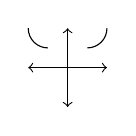
\begin{tikzpicture}
  \draw[<->] (-.5,0) -- (.5,0);
  \draw[<->] (0,-.5) -- (0,.5);
  \draw[in=270,out=0] (.25,.25) to (.5,.5);
  \draw[in=270,out=180] (-.25,.25) to (-.5,.5);
\end{tikzpicture}
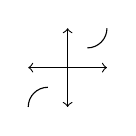
\begin{tikzpicture}
  \draw[<->] (-.5,0) -- (.5,0);
  \draw[<->] (0,-.5) -- (0,.5);
  \draw[in=270,out=0] (.25,.25) to (.5,.5);
  \draw[in=90,out=180] (-.25,-.25) to (-.5,-.5);
\end{tikzpicture}
\end{minipage}~
\begin{minipage}{40pt}
\[
y=-x^n
\]
$n$ is even\vspace{5pt}
\[
y=-x^n
\]
$n$ is odd
\end{minipage}
\begin{minipage}{30pt}
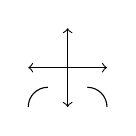
\begin{tikzpicture}
  \draw[<->] (-.5,0) -- (.5,0);
  \draw[<->] (0,-.5) -- (0,.5);
  \draw[in=90,out=0] (.25,-.25) to (.5,-.5);
  \draw[in=90,out=180] (-.25,-.25) to (-.5,-.5);
\end{tikzpicture}
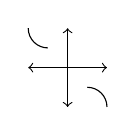
\begin{tikzpicture}
  \draw[<->] (-.5,0) -- (.5,0);
  \draw[<->] (0,-.5) -- (0,.5);
  \draw[in=90,out=0] (.25,-.25) to (.5,-.5);
  \draw[in=270,out=180] (-.25,.25) to (-.5,.5);
\end{tikzpicture}
\end{minipage}
\end{minipage}}
\fbox{\begin{minipage}{119pt}
\centering $m\times n$ matrix
\[\left[
  \begin{array}{ccccc}
    a_{11} & a_{12} & \cdots & a_{1n} \\
    a_{21} & a_{22} & \cdots & a_{2n} \\
    \vdots & \vdots & \ddots & \vdots \\
    a_{m1} & a_{m2} & \cdots & a_{mn} \\ % worked out beautifully, huh? Completely unintentional.
  \end{array}
\right]\]
\end{minipage}}

\fbox{\begin{minipage}{207pt}
\centering $y=\sin x$ in red; $y=\cos x$ in blue
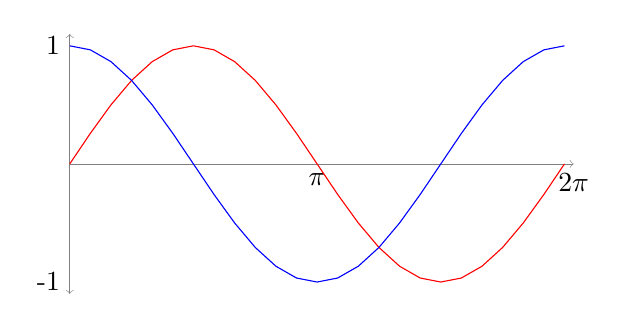
\begin{tikzpicture}[yscale=1.5]
\draw [help lines, ->] (0,0) -- (6.4,0);
\node [below] at (6.4,0) {$2\pi$};
\node [below] at (pi,0) {$\pi$};
\node [left] at (0,1) {1};
\node [left] at (0,-1) {-1};
\draw [help lines, <->] (0,-1.1) -- (0,1.1);
\draw [red,domain=0:2*pi] plot (\x, {sin(\x r)});
\draw [blue, domain=0:2*pi] plot (\x, {cos(\x r)});

\end{tikzpicture}
\end{minipage}}
\fbox{ \begin{minipage}{110pt}
\centering sin/cos Graph Properties

\raggedright If in form:
\[
y=a\sin k(x-b)
\]
amplitude  $|a|$, period  $2\pi/k$, phase shift $b$
\end{minipage}}
\fbox{ \begin{minipage}{193pt}
    \centering Allowed row operations
    \begin{enumerate}
    \item Add a multiple of one row to another
    \item Multiply a row by a nonzero constant
    \item Interchange two rows
    \end{enumerate}
\end{minipage}}
\fbox{ \begin{minipage}{250pt}
\[
\textrm{If }
\left\{\begin{array}{l}
    ax + by = r \\
    cx + dy = s \\
  \end{array}\right.
  \textrm{ then }
  x = \frac{\left|\begin{array}{cc}
  r & b \\
  s & d \\
    \end{array}\right|}
  {\left|\begin{array}{cc}
  a & b \\
  c & d \\
    \end{array}\right|}
  \textrm{ and }
  y = \frac{\left|\begin{array}{cc}
    a & r \\
    c & s \\
    \end{array}\right|}
  {\left|\begin{array}{cc}
  a & b \\
  c & d \\
    \end{array}\right|}
\]
\end{minipage}}
\fbox{ \begin{minipage}{80pt}
    \centering Parabola
\[
x^2 = 4py
\]
\raggedright    $V(0,0)$, $F(0,p)$, directrix $y=-p$
\end{minipage}}
\fbox{ \begin{minipage}{106pt}
\centering Ellipse
\[
\frac{x^2}{(a\textrm{ or }b)^2} + \frac{y^2}{(a\textrm{ or }b)^2} = 1
\] \[
c^2 = a^2 - b^2
\]
\end{minipage}}
\fbox{ \begin{minipage}{53pt}
\centering Eccentricity
\[
e = \frac ca,
\]
\end{minipage}}

\fbox{ \begin{minipage}{55pt}
\centering Hyperbola
\[
\frac{x^2}{ab^2} - \frac{y^2}{b^2} = 1
\] \[
c^2 = a^2 + b^2
\]
\end{minipage}}
\fbox{ \begin{minipage}{53pt}
\centering General Conic
\[
\frac{d(P,F)}{d(P,l)}=e
\]
\end{minipage}}
\fbox{ \begin{minipage}{100pt}
\centering Polar Conics
\[
r = \frac{ed}{1\pm e(\cos\textrm{ or }\sin)\theta}
\]
\end{minipage}}
\fbox{ \begin{minipage}{53pt}
\centering Derivative Formula
\[
f^{-1} (a) = \lim_{h \to 0} \frac{ f(a+h)-f(a) }{h} 
\]
\end{document}
